\begin{table}[htbp]
  \caption{Park value formula and its per plate appearance in each team}
  \label{tab:PF_PFPA} 
  \centering
  \resizebox{\columnwidth}{!}{
    \begin{tabular}{|l|c|c|c|c|c|c|c|c|c|}
      \hline
      TEAM & PF & PFPA & TEAM & PF & PFPA & TEAM & PF & PFPA\\ 
      \hline
     ARI & 1.05 & 0.006 & ATL & 1.00 & 0.000 & BAL & 1.01 & 0.001\\
     BOS & 1.04 & 0.005 & CHA & 1.04 & 0.005 & CHN & 1.04 & 0.005\\
     CIN & 1.02 & 0.002 & CLE & 1.00 & 0.000 & COL & 1.09 & 0.011\\
     DET & 1.00 & 0.000 & FLA & 0.98 & -0.002 & HOU & 0.99 & -0.001\\
     KC & 1.00 & 0.000 & LAA & 0.98 & -0.002 & LAN & 0.99 & -0.001\\
     MIL & 1.00 & 0.000 & MIN & 1.00 & 0.000 & NYA & 1.00 & 0.000\\
     NYN & 0.97 & -0.004 & OAK & 0.98 & -0.002 & PHI & 1.02 & 0.002\\
     PIT & 0.98 & -0.002 & SD & 0.92 & -0.010 &SEA & 0.97 & -0.004 \\
     SF & 1.01 & 0.001 & STL & 0.98 & -0.002 &TB & 0.99 & -0.001\\
     TEX & 1.03 & 0.004 & TOR & 1.02 & 0.002 & WAS & 1.01 & 0.001\\

    \end{tabular}
  }
  \cite{web:Wyers:Part3}
\end{table}

\begin{figure}[tbp]
  \centering
  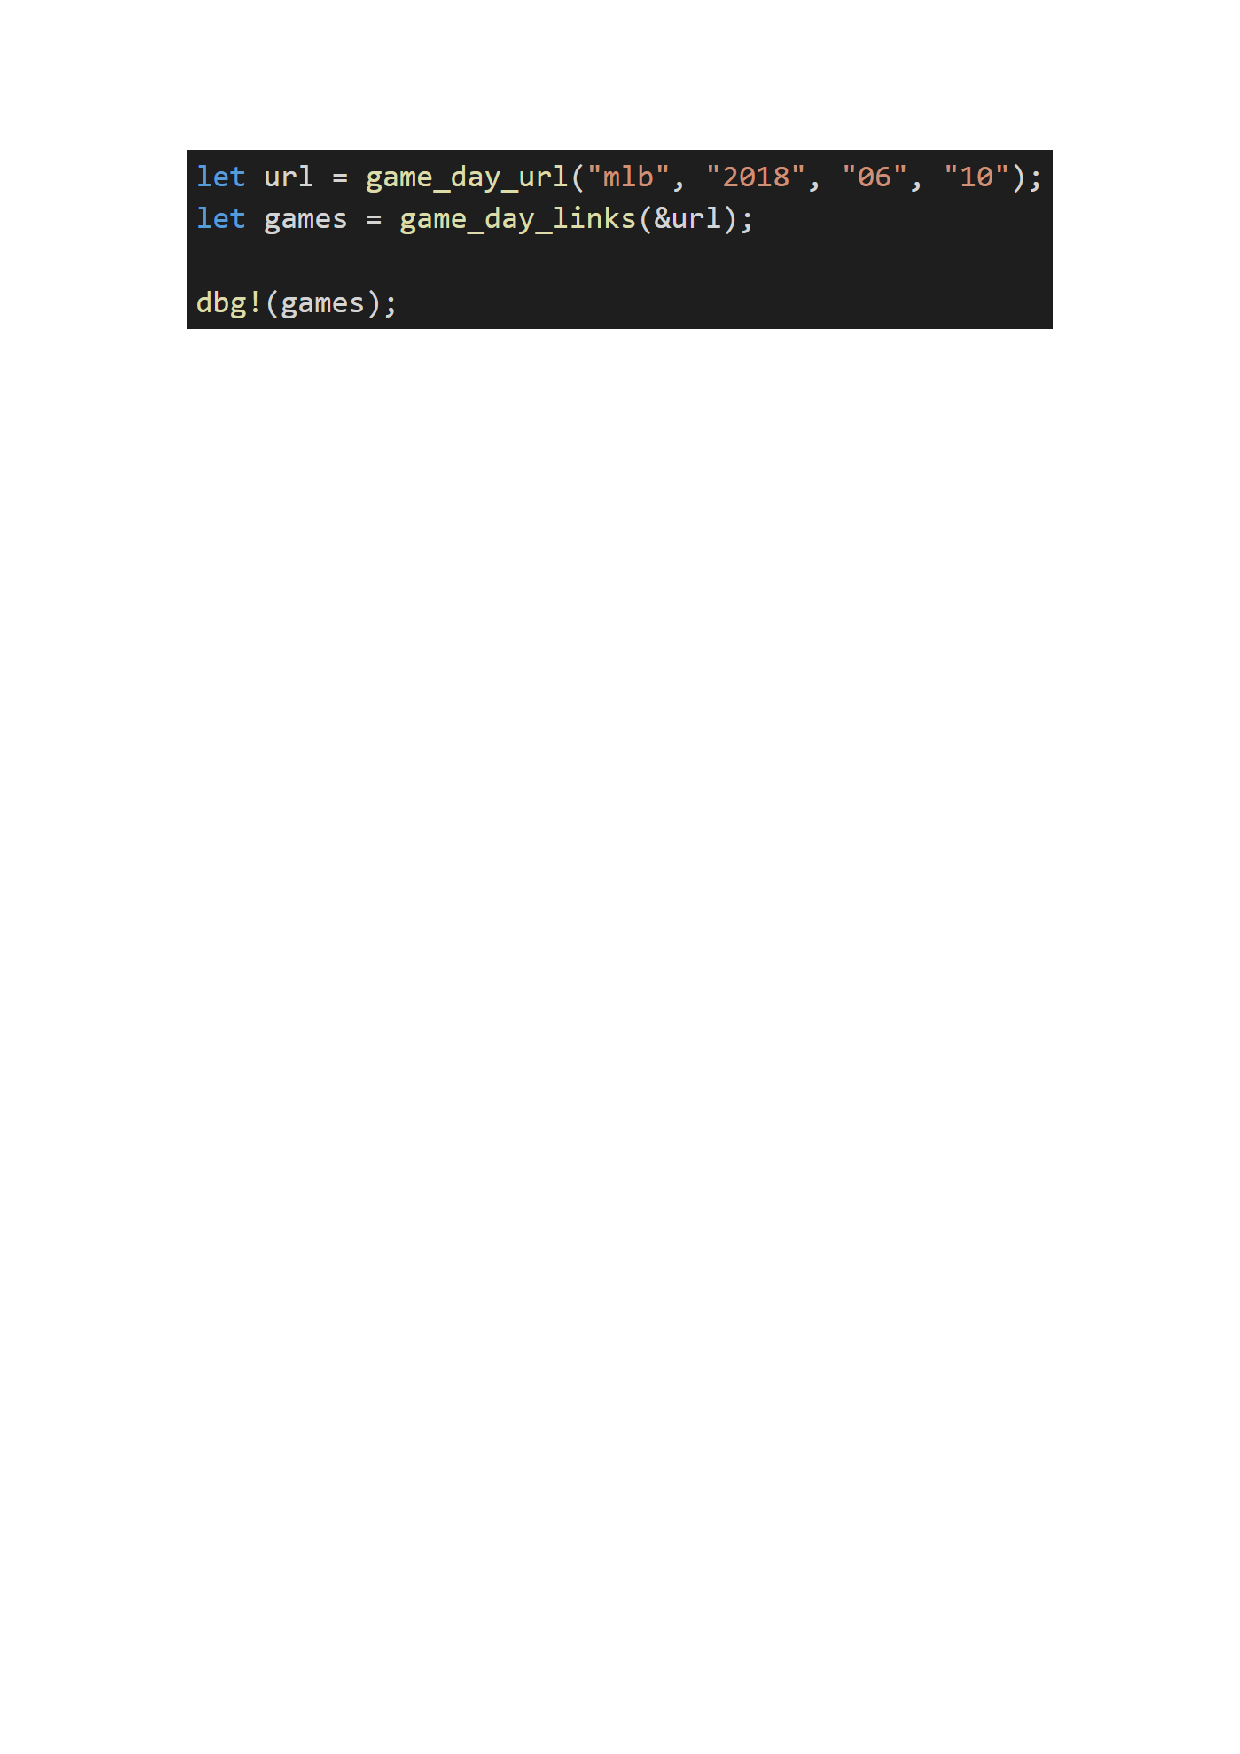
\includegraphics[width=\textwidth]{baseballcode.pdf}
  \caption{code for addressing stats 2008 baseball team}
  \label{fig:baseballcode}
\end{figure}

\begin{table}[h]
  \caption{full nitty-gritty}
  \label{tab:ng} 
  \centering
  \resizebox{\columnwidth}{!}{
  \begin{tabular}{|l|c|c|c|c|c|c|}
    \hline
    Pos & RZR & OOZ_INN & Run/Play & BIZ/30 & PAdj\\
    \hline
    1B & 0.739422 & 0.030305 & 0.798 & 219 & -12.5\\
    2B & 0.821831 & 0.026007 & 0.754 & 426 & 2.5\\
    3B & 0.696536 & 0.038408 & 0.8 & 354.1333 & 2.5\\
    CF & 0.921688 & 0.067393 & 0.842 & 349.0333 & 2.5\\
    LF & 0.882837 & 0.04453 & 0.831 & 275.4 & -7.5\\
    RF & 0.899098 & 0.048531 & 0.843 & 292.0333 & -7.5\\
    SS & 0.828403 & 0.037678 & 0.753 & 424.8333 & 7.5\\
  \end{tabular}
  }
\cite*{web:Wyers:Part3}
\end{table}

\begin{table}[htbp]
  \caption{Top 10 Player in 2008}
  \label{tab:top} 
  \centering
  \begin{tabular}{|l|l|c|c|c|c|c|}
     \hline
     \textbf{Last Name} & \textbf{First Name} & \textbf{Offesne} & \textbf{Bonus} & \textbf{Defense} & \textbf{Total} & \textbf{WAR}\\
     \hline
     Pujols & Albert & 73.3 & 18.3 & 16.7 & 108.4 & 10.8\\
     Jones & Chipper & 51.5 & 15.3 & 18.1 & 84.9 & 8.5\\
     Utley & Chase & 33.6 & 20.2 & 30.0 & 83.7 & 8.4\\
     Berkman & Lance & 49.5 & 19.0 & 12.6 & 81.0 & 8.1\\
     Rodriguez & Alex & 39.0 & 21.2 & 14.3 & 74.4 & 7.4\\
     Teixeira & Mark & 45.5 & 21.2 & 7.2 & 74.0 & 7.4\\
     Ramirez & Hanley & 40.8 & 19.8 & 9.6 & 70.2 & 7.0\\
     Wright & David A & 41.0 & 21.0 & 7.3 & 69.4 & 6.9\\
     Beltran & Carlos & 30.4 & 20.2 & 16.8 & 67.4 & 6.7\\
     Sizemore & Grady & 30.1 & 26.6 & 8.1 & 64.8 & 6.5\\
    \hline
  \end{tabular}
\end{table}


\begin{table}[htbp]
  \caption{Buttom 10 Players in 2008}
  \label{tab:buttom} 
  \centering
  \begin{tabular}{|l|l|c|c|c|c|c|}
     \hline
     \textbf{Last Name} & \textbf{First Name} & \textbf{Offense} & \textbf{RepBonus} & \textbf{Defense} & \textbf{Total} & \textbf{WAR}\\
     \hline
     Wilkerson & Brad & -13.9 & 11.0 & -9.4 & -12.3 & -1.2\\
     Balentien & Wladimir R & -16.1 & 9.3 & -6.0 & -12.9 & -1.3\\
     Jacobs & Mike & 5.4 & 14.8 & -31.5 & -11.3 & -1.1\\
     Matthews Jr. & Gary & -12.6 & 17.0 & -16.4 & -11.9 & -1.2\\
     Patterson & Corey & -29.4 & 11.2 & 4.7 & -13.5 & -1.4\\
     Lamb & Mike & -15.6 & 9.6 & -8.5 & -14.4 & -1.4\\
     Francoeur & Jeff B & -26.0 & 18.7 & -4.6 & -11.9 & -1.2\\
     Pena & Tony F & -30.4 & 8.4 & 6.2 & -15.8 & -1.6\\
     Guillen & Jose & -9.7 & 22.6 & -28.3 & -15.4 & -1.5\\
     Gload & Ross & -15.4 & 14.9 & -20.1 & -20.6 & -2.1\\
    \hline
  \end{tabular}
\end{table}


\begin{table}[htbp]
  \caption{Baseball Batting Statistics}
  \label{tab:discription} 
  \centering
  \begin{tabular}{|l|l|}
     \hline
     \textbf{Variable} & \textbf{Description}\\
     \hline
     $AB$ & At bats\\
     $AVG$ & Batting average\\
     $H$ & Hits\\
     $K$ & Strikeouts\\
     $HR$ & Home Run\\
     $BABIP$ & Batting Average on Balls in Play\\
     $SF$ & Sacrifice flies\\
    \hline
  \end{tabular}
\end{table}